\chapter{Specifikacija programske potpore}
		
	\section{Funkcionalni zahtjevi}			
			
			\noindent \textbf{Dionici:}
			
			\begin{packed_enum}
				
				\item Korisnici
					\begin{packed_enum}
						\item  Neregistrirani
						\item  Registrirani
					\end{packed_enum}
				\item Moderator
				\item Razvojni tim
				
			\end{packed_enum}
			
			\noindent \textbf{Aktori i njihovi funkcionalni zahtjevi:}
			
			
			\begin{packed_enum}
				\item  \underbar{Neregistrirani/neprijavljeni korisnik (inicijator) može:}
				
				\begin{packed_enum}
					
					\item pregledati objavljene oglase pod nadimkom
					\item filtrirati oglase po smjeru, kolegiju i kategoriji
					\item pregledati rejting listu studenata- pomagača pod njihovim nadimkom
					\item se registrirati u sustav, stvoriti novi korisnički račun za koji su mu potrebni  ime, prezime, korisničko ime, avatara, e-mail i lozinka
					
				\end{packed_enum}
			
				\item  \underbar{Registrirani korisnik (inicijator) može:}
				
				\begin{packed_enum}
					
					\item javljati se na objavljene oglase
					\item objavljivati oglase
					\item ocjenjivati studente-pomagače
					\item pregledavati i mijenjati osobne podatke
					\item pregledavati i mijenjati svoje aktivne oglase
					\item obrisati svoje aktivne oglase
					\item promijeniti status upita na oglas (prihvaćen ili odbijen)
					
				\end{packed_enum}
			
				\item  \underbar{Moderator (inicijator) može:}
				
				\begin{packed_enum}
					
					\item uklanjati nepravilne i neprikladne oglase
					\item dodavati, mijenjati i brisati kolegije
					\item pretraživati kolegije
					
				\end{packed_enum}
			
				\item  \underbar{Baza podataka (sudionik):}
				
				\begin{packed_enum}
					
					\item pohranjuje sve podatke o korisnicima 
					\item pohranjuje sve podatke o oglasima
					\item pohranjuje kolegije
					
				\end{packed_enum}
			\end{packed_enum}
			
			\eject 
			
			
				
			\subsection{Obrasci uporabe}
				
				\subsubsection{Opis obrazaca uporabe}

					\noindent \underbar{\textbf{UC1 - Pregled objavljenih oglasa}}
					\begin{packed_item}
	
						\item \textbf{Glavni sudionik: }Neregistrirani korisnik
						\item  \textbf{Cilj:} Mogućnost pregleda objavljenih oglasa
						\item  \textbf{Sudionici:} Baza podataka
						\item  \textbf{Preduvjet:} -
						\item  \textbf{Opis osnovnog tijeka:}
						
						\item[] \begin{packed_enum}
							\item Dohvaćanje aktivnih oglasa iz baze podataka
							\item Prikaz aktivnih oglasa neregistriranom korisniku
						\end{packed_enum}
						
						\item  \textbf{Opis mogućih odstupanja:}
						
						\item[] \begin{packed_item}
	
							\item[1.a] Nema aktivnih oglasa
							\item[] \begin{packed_enum}
								\item Sustav obavještava korisnika da nema aktivnih oglasa
							\end{packed_enum}
							
						\end{packed_item}
					\end{packed_item}
				
				
					\noindent \underbar{\textbf{UC2 - Pregled rejting-liste}}
					\begin{packed_item}
						
						\item \textbf{Glavni sudionik: }Neregistrirani korisnik
						\item  \textbf{Cilj:} Mogućnost pregleda rejting-liste studenata pomagača pod nadimcima
						\item  \textbf{Sudionici:} Baza podataka
						\item  \textbf{Preduvjet:} -
						\item  \textbf{Opis osnovnog tijeka:}
						
						\item[] \begin{packed_enum}
							\item Neregistrirani korisnik zahtjeva prikaz liste 10 najboljih student-pomagača
							\item Lista student-pomagača dohvaća se iz baze podataka
							\item Rangiranje studenata-pomagača unutar web aplikacije
							\item Prikaz liste neregistriranom korisniku
						\end{packed_enum}
						
						\item  \textbf{Opis mogućih odstupanja:}
						
						\item[] \begin{packed_item}
							
							\item[2.a] Nema registriranih student-pomagača
							\item[] \begin{packed_enum}
								\item Sustav obavještava korisnika da ne postoje registrirani student-pomagači
							\end{packed_enum}
							
							\item[3.a] Studente-pomagače nije moguće rangirati
							\item[] \begin{packed_enum}
								\item Sustav prikazuje praznu rejting listu
							\end{packed_enum}
							
						\end{packed_item}
					\end{packed_item}
				
				
				
					\noindent \underbar{\textbf{UC3 - Filtriranje oglasa}}
					\begin{packed_item}
						
						\item \textbf{Glavni sudionik: }Neregistrirani korisnik
						\item  \textbf{Cilj:} Mogućnost filtriranja oglasa po smjeru, kolegiju i kategoriji
						\item  \textbf{Sudionici:} Baza podataka, Web aplikacija
						\item  \textbf{Preduvjet:} Korisniku se prikazuju aktivni oglasi
						\item  \textbf{Opis osnovnog tijeka:}
						
						\item[] \begin{packed_enum}
							\item Korisnik odabire opciju smjer(računarstvo ili elektrotehnika), kolegij i/ili kategoriju(laboratorijska vježba, blic, gradivo, kontinuirani ispit ili ispitni rok)
							\item Korisnik odabire opciju „Filtriraj“ 
							\item Web aplikacija filtrira listu oglasa po danim kriterijima i osvježava prikaz filtriranih oglasa
						\end{packed_enum}
						
						\item  \textbf{Opis mogućih odstupanja:}
						
						\item[] \begin{packed_item}
							
							\item[2.a] Korisnik filtrira, a nije izabrao nijednu od opcija (smjer, kolegij, kategorija):
							\item[] \begin{packed_enum}
								\item Prikazuju se svi oglasi
							\end{packed_enum}
							
						\end{packed_item}
					\end{packed_item}
				
					
					\noindent \underbar{\textbf{UC4 - Registracija}}
					\begin{packed_item}
						
						\item \textbf{Glavni sudionik: }Neregistrirani korisnik
						\item  \textbf{Cilj:} Stvoriti korisnički račun za pristup sustavu
						\item  \textbf{Sudionici:} Baza podataka
						\item  \textbf{Preduvjet:} -
						\item  \textbf{Opis osnovnog tijeka:}
						
						\item[] \begin{packed_enum}
							\item Korisnik odabire opciju za registraciju
							\item Korisnik unosi podatke potrebne za registraciju
							\item Aplikacija provjerava ispravni format unesenih podataka
							\item Podaci se upisuju u bazu podataka
							\item Korisniku se šalje e-mail pošta za potvrdu registracije računa
						\end{packed_enum}
						
						\item  \textbf{Opis mogućih odstupanja:}
						
						\item[] \begin{packed_item}
							
							\item[2.a] Korisnik je unio već zauzeto korisničko ime i/ili e-mail ili je unio e-mail koji nije iz fer.hr domene 
							\item[] \begin{packed_enum}
								\item Sustav obavještava korisnika o pogrešci te briše polje lozinke
							\end{packed_enum}

						\end{packed_item}
					\end{packed_item}
				
	
				
				\noindent \underbar{\textbf{UC5 - Pregled svojih objavljenih oglasa}}
				\begin{packed_item}
					
					\item \textbf{Glavni sudionik: }Registrirani korisnik
					\item  \textbf{Cilj:} Pregledati sve svoje objavljene oglase  
					\item  \textbf{Sudionici:} Baza podataka
					\item  \textbf{Preduvjet:} Korisnik je prijavljen
					\item  \textbf{Opis osnovnog tijeka:}
					
					\item[] \begin{packed_enum}
						\item Korisnik odlazi na rubriku „Moji objavljeni oglasi“
						\item Aplikacija šalje upit bazi za prikaz svih aktivnih oglasa
						\item Aktivni oglasi prikazuju se korisniku
					\end{packed_enum}
					
					\item  \textbf{Opis mogućih odstupanja:}
					
					\item[] \begin{packed_item}
						
						\item[2.a] Nema aktivnih oglasa za prikaz
						\item[] \begin{packed_enum}
							\item Aplikacija ispisuje poruku „Nema oglasa za prikaz“ 
						\end{packed_enum}
						
					\end{packed_item}
				\end{packed_item}
				
				
					\noindent \underbar{\textbf{UC6 - Objava oglasa }}
					\begin{packed_item}
						
						\item \textbf{Glavni sudionik: }Registrirani korisnik
						\item  \textbf{Cilj:} Objaviti oglas  
						\item  \textbf{Sudionici:} Baza podataka
						\item  \textbf{Preduvjet:} Korisnik je prijavljen
						\item  \textbf{Opis osnovnog tijeka:}
						
						\item[] \begin{packed_enum}
							\item Korisnik odabire opciju „Objavi oglas“
							\item Unosi sadržaj svog oglasa (naslov, opis, kolegij, kategorija) 
							\item Podaci se upisuju u bazu podataka
						\end{packed_enum}
						
						\item  \textbf{Opis mogućih odstupanja:}
						
						\item[] \begin{packed_item}
							
							\item[2.a] Korisnik nije unio sve obvezne komponente oglasa
							\item[] \begin{packed_enum}
								\item Sustav obavještava korisnika o podacima koji nisu ispravno uneseni
							\end{packed_enum}
							
						\end{packed_item}
					\end{packed_item}
				
				
					
				
				
					\noindent \underbar{\textbf{UC7 - Izmjena objavljenih oglasa}}
					\begin{packed_item}
						
						\item \textbf{Glavni sudionik: }Registrirani korisnik
						\item  \textbf{Cilj:} Izmijeniti značajke oglasa   
						\item  \textbf{Sudionici:} Baza podataka
						\item  \textbf{Preduvjet:} Korisnik je prijavljen i oglas je objavljen
						\item  \textbf{Opis osnovnog tijeka:}
						
						\item[] \begin{packed_enum}
							\item Korisnik odlazi na rubriku „Moji objavljeni oglasi“
							\item Korisnik odabire oglas koji želi izmijeniti
							\item Korisnik odabere opciju za izmjenu oglasa
							\item Korisnik izmjenjuje željene značajke oglasa
							\item Korisnik sprema promjene
							\item Baza podataka se ažurira
						\end{packed_enum}
						
						\item  \textbf{Opis mogućih odstupanja:}
						
						\item[] \begin{packed_item}
							
							\item[4.a] Korisnik je obrisao sav sadržaj oglasa i pokušava ga ponovno objaviti 
							\item[] \begin{packed_enum}
								\item Sustav obavještava korisnika da ne može objaviti prazan oglas
							\end{packed_enum}
							
						\end{packed_item}
					\end{packed_item}
					
					
					\noindent \underbar{\textbf{UC8 - Brisanje oglasa}}
					\begin{packed_item}
						
						\item \textbf{Glavni sudionik: }Registrirani korisnik
						\item  \textbf{Cilj:} Obrisati objavljeni oglas  
						\item  \textbf{Sudionici:} Baza podataka
						\item  \textbf{Preduvjet:} Korisnik je prijavljen i oglas je objavljen
						\item  \textbf{Opis osnovnog tijeka:}
						
						\item[] \begin{packed_enum}
							\item Korisnik odlazi na rubriku „Moji objavljeni oglasi“
							\item Korisnik odabire oglas koji želi obrisati
							\item Korisnik stisne gumb „Obriši oglas“
							\item Sustav izbacuje skočni prozor s pitanjem „Jeste li sigurni da želite obrisati ovaj oglas?“
							\item Korisnik odabire „Da“ ili „Ne“
							\item Baza podataka se ažurira
						\end{packed_enum}
						
					\end{packed_item}
				
				
					\noindent \underbar{\textbf{UC9 - Odgovaranje na oglase}}
					\begin{packed_item}
						
						\item \textbf{Glavni sudionik: }Registrirani korisnik
						\item  \textbf{Cilj:} Odgovoriti na objavljeni oglas   
						\item  \textbf{Sudionici:} Baza podataka
						\item  \textbf{Preduvjet:} Korisnik je prijavljen i oglas je objavljen
						\item  \textbf{Opis osnovnog tijeka:}
						
						\item[] \begin{packed_enum}
							\item Korisnik bira oglas na koji želi odgovoriti
							\item Korisnik upisuje svoj odgovor
							\item Sustav šalje e-mail objavljivaču oglasa
							\item Daljnja komunikacija odvija se e-mailom između korisnika i studenta-pomagača
						\end{packed_enum}
						
					\end{packed_item}
				
				
					\noindent \underbar{\textbf{UC10 - Pregled statusa upita}}
					\begin{packed_item}
						
						\item \textbf{Glavni sudionik: }Registrirani korisnik
						\item  \textbf{Cilj:} Pogledati status poslanog upita  
						\item  \textbf{Sudionici:} Baza podataka
						\item  \textbf{Preduvjet:} Korisnik je prijavljen i poslan je upit na oglas
						\item  \textbf{Opis osnovnog tijeka:}
						
						\item[] \begin{packed_enum}
							\item Korisnik odlazi na rubriku „Status mojih upita“
							\item Aplikacija šalje upit bazi za prikaz statusa upita
							\item Korisniku se prikazuje status njegovog upita (prihvaćen, odbijen ili u tijeku)
						\end{packed_enum}
						
					\end{packed_item}
				
				
					\noindent \underbar{\textbf{UC11 - Promjena statusa upita}}
					\begin{packed_item}
						
						\item \textbf{Glavni sudionik: }Registrirani korisnik
						\item  \textbf{Cilj:} Promijeniti status primljenog upita  
						\item  \textbf{Sudionici:} Baza podataka
						\item  \textbf{Preduvjet:} Korisnik je prijavljen i primljen je upit na oglas
						\item  \textbf{Opis osnovnog tijeka:}
						
						\item[] \begin{packed_enum}
							\item Korisnik odlazi na rubriku „Upiti na moje oglase“
							\item Aplikacija šalje upit bazi za prikaz upita
							\item Korisniku se prikazuje upiti na njegove oglase
							\item Korisnik prihvaća ili odbija upit na oglas
							\item Baza podataka se ažurira
						\end{packed_enum}
						
					\end{packed_item}
				
				
					\noindent \underbar{\textbf{UC12 - Ocjenjivanje pomagača}}
					\begin{packed_item}
						
						\item \textbf{Glavni sudionik: }Registrirani korisnik
						\item  \textbf{Cilj:} Ocijeniti studenta-pomagača  
						\item  \textbf{Sudionici:} Baza podataka
						\item  \textbf{Preduvjet:} Korisnik je prijavljen i objavljen je bar jedan oglas na temelju kojeg se pomagač ocjenjuje
						\item  \textbf{Opis osnovnog tijeka:}
						
						\item[] \begin{packed_enum}
							\item Korisnik nakon pozitivnog odgovora ocjenjuje studenta-pomagača 
							\item Korisnik odabire ocjenu koju mu želi dati 
							\item Ažurira se rejting-lista i srednja ocjena studenta-pomagača
							\item Baza podataka se ažurira
						\end{packed_enum}
						
					\end{packed_item}
				
				
					\noindent \underbar{\textbf{UC13 - Izmjena informacija o profilu}}
					\begin{packed_item}
						
						\item \textbf{Glavni sudionik: }Registrirani korisnik
						\item  \textbf{Cilj:} Izmijeniti informacije o svom profilu 
						\item  \textbf{Sudionici:} Baza podataka
						\item  \textbf{Preduvjet:} Korisnik je prijavljen
						\item  \textbf{Opis osnovnog tijeka:}
						
						\item[] \begin{packed_enum}
							\item Korisnik odabire opciju za promjenu svojih podataka 
							\item Korisnik mijenja svoje podatke 
							\item Korisnik sprema promjene
							\item Baza podataka se ažurira
						\end{packed_enum}
					
					\end{packed_item}
				
				
					\noindent \underbar{\textbf{UC14 - Uklanjanje nepravilnih oglasa}}
					\begin{packed_item}
						
						\item \textbf{Glavni sudionik: }Moderator
						\item  \textbf{Cilj:} Ukloniti nepravilne ili neprikladne oglase
						\item  \textbf{Sudionici:} Baza podataka
						\item  \textbf{Preduvjet:} Korisnik je prijavljen i dodijeljena su mu prava moderatora
						\item  \textbf{Opis osnovnog tijeka:}
						
						\item[] \begin{packed_enum}
							\item Moderator pregledava oglase i utvrđuje nepravilnosti
							\item Moderator piše objašnjenje za brisanje oglasa 
							\item Moderator odabire opciju „Obriši oglas”
							\item Korisniku se šalje e-mail s objašnjenjem zašto je njegov oglas uklonjen
							\item Baza podataka se ažurira
							
						\end{packed_enum}
						
						\item  \textbf{Opis mogućih odstupanja:}
						
						\item[] \begin{packed_item}
							
							\item[1.a] Nema aktivnih oglasa
							\item[] \begin{packed_enum}
								\item Sustav obavještava moderatora da nema aktivnih oglasa
							\end{packed_enum}
							
						\end{packed_item}
					\end{packed_item}
				
				
					\noindent \underbar{\textbf{UC15 - Dodavanje kolegija}}
					\begin{packed_item}
						
						\item \textbf{Glavni sudionik: }Moderator
						\item  \textbf{Cilj:} Dodati novi kolegij
						\item  \textbf{Sudionici:} Baza podataka
						\item  \textbf{Preduvjet:} Korisnik je prijavljen i dodijeljena su mu prava moderatora
						\item  \textbf{Opis osnovnog tijeka:}
						
						\item[] \begin{packed_enum}
							\item Moderator odabire opciju „Dodaj kolegija”
							\item Moderator unosi podatke o novom kolegiju  
							\item Moderator odabire opciju „Unesi kolegij”
							\item Podaci se upisuju u bazu podataka
							
						\end{packed_enum}
						
						\item  \textbf{Opis mogućih odstupanja:}
						
						\item[] \begin{packed_item}
							
							\item[3.a] Kolegij već postoji u bazi podataka
							\item[] \begin{packed_enum}
								\item Sustav obavještava moderatora o neuspješnom unosu kolegija u bazu podataka
							\end{packed_enum}
							
						\end{packed_item}
					\end{packed_item}
				
				
					\noindent \underbar{\textbf{UC16 - Kategorizacija kolegija}}
					\begin{packed_item}
						
						\item \textbf{Glavni sudionik: }Moderator
						\item  \textbf{Cilj:} Kategorizirati kolegij po smjerovima
						\item  \textbf{Sudionici:} Baza podataka
						\item  \textbf{Preduvjet:} Korisnik je prijavljen i dodijeljena su mu prava moderatora, kolegij postoji u bazi podataka
						\item  \textbf{Opis osnovnog tijeka:}
						
						\item[] \begin{packed_enum}
							\item Moderator odabire prikaz liste kolegija
							\item Moderator odabire kolegij iz liste kolegija 
							\item Moderator odabire smjer (jedan od preddiplomskih ili diplomskih smjerova)
							\item Podaci se upisuju u bazu podataka
							
						\end{packed_enum}
						
					\end{packed_item}
				
				\eject
					
				\subsubsection{Dijagrami obrazaca uporabe}
				
					\begin{figure}[H]
						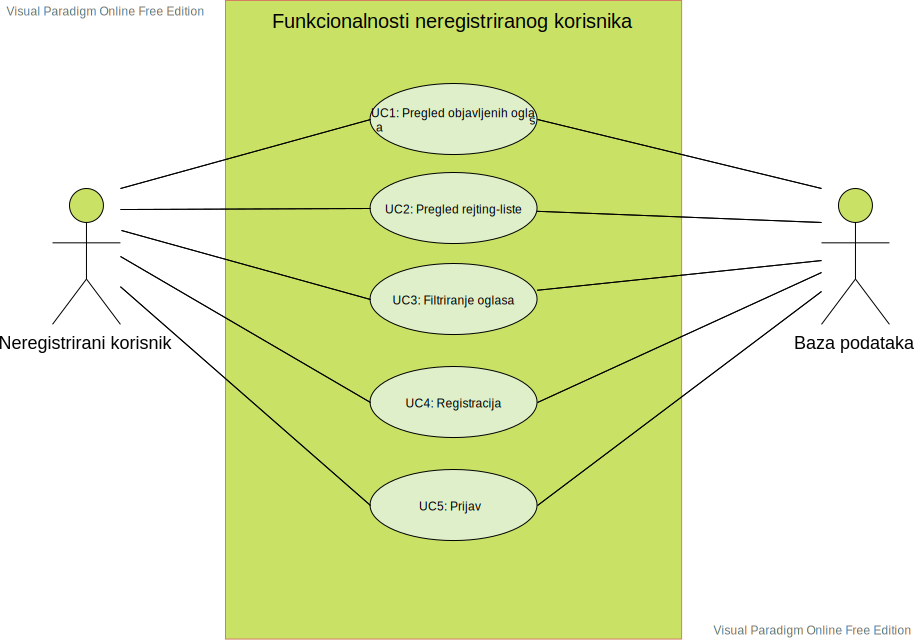
\includegraphics[scale=0.63]{dijagrami/UC_NeregistriranKorisnik.PNG}
						\centering
						\caption{Dijagram obrasca uporabe, funkcionalnosti neregistriranog korisnika}
						\label{fig:UC_NeregistriranKorisnik}
					\end{figure}
				
					\begin{figure}[H]
						\includegraphics[scale=0.7]{dijagrami/UC_RegistriraniKorisnik.PNG}
						\centering
						\caption{Dijagram obrasca uporabe, funkcionalnosti registriranog korisnika}
						\label{fig:UC_RegistriranKorisnik}
					\end{figure}				
				
					\begin{figure}[H]
						\includegraphics[scale=0.9]{dijagrami/UC_Moderator.PNG}
						\centering
						\caption{Dijagram obrasca uporabe, funkcionalnosti moderatora}
						\label{fig:UC_Moderator}
					\end{figure}
					
			\eject
				
			\subsection{Sekvencijski dijagrami}
			
					\noindent \textbf{Obrazac uporabe UC4 - Registracija}
					
					\noindent Korisnik otvara formu za registraciju i upisuje svoje podatke. Poslužitelj provjerava je li čitava forma popunjena i nalazi li se e-mail u FER-ovoj domeni. Poslužitelj pohranjuje podatke u bazu podataka.  Ukoliko su zauzeti korisničko ime ili e-mail adresa sustav obavještava korisnika o tome i ispisuje poruku.
					
					\begin{figure}[H]
						\includegraphics[scale=0.7]{dijagrami/SD_registracija.png}
						\centering
						\caption{Sekvencijski dijagram za UC4}
						\label{fig:SD_registracija}
					\end{figure}
					
			\eject
			
					\noindent \textbf{Obrazac uporabe UC7 - Izmjena objavljenih oglasa}
					
					\noindent Korisnik šalje zahtjev za prikaz aktivnih oglasa. Poslužitelj dohvaća oglase i prikazuje ih korisniku. Korisnik mijenja neke od komponenata oglasa. Poslužitelj provjerava je li koja od komponenata prazna, tj. izbrisana. Ako je promjena validna, ona se pohranjuje u bazu podataka te korisnik dobiva poruku „Promjene unesene“.
					
					\begin{figure}[H]
						\includegraphics[scale=0.7]{dijagrami/SD_IzmjenaOglasa.png}
						\centering
						\caption{Sekvencijski dijagram za UC7}
						\label{fig:SD_IzmjenaOglasa}
					\end{figure}
					
			\eject
			
					\noindent \textbf{Obrazac uporabe UC13 - Izmjena informacija o profilu}
					
					\noindent Korisnik šalje zahtjev za prikaz aktivnih oglasa. Poslužitelj dohvaća oglase i prikazuje ih korisniku. Korisnik mijenja neke od komponenata oglasa. Poslužitelj provjerava je li koja od komponenata prazna, tj. izbrisana. Ako je promjena validna, ona se pohranjuje u bazu podataka te korisnik dobiva poruku „Promjene unesene“. Ukoliko dođe do greške u obradi zahtjeva sustav obavještava korisnika da promjene nisu unesene.
					
					\begin{figure}[H]
						\includegraphics[scale=0.7]{dijagrami/SD_IzmjenaInf.png}
						\centering
						\caption{Sekvencijski dijagram za UC13}
						\label{fig:SD_IzmjenaInf}
					\end{figure}
					
			\eject
			
					\noindent \textbf{Obrazac uporabe UC14 - Uklanjanje nepravilnih oglasa}
					
					\noindent Moderator šalje zahtjev za prikaz aktivnih oglasa. Poslužitelj dohvaća oglase i prikazuje ih korisniku. Ukoliko ne postoje aktivni oglasi, moderator dobiva poruku „Nema aktivnih oglasa za prikaz“. Moderator briše oglas i piše razlog zašto je oglas obrisan. Razlog se šalje korisniku na mail te se oglas briše iz baze podataka. Sustav moderatoru vraća prikaz aktivnih oglasa. Ukoliko su svi oglasi obrisani, moderator dobiva poruku „Nema aktivnih oglasa za prikaz“.
					
					\begin{figure}[H]
						\includegraphics[scale=0.7]{dijagrami/SD_Uklanjanje.png}
						\centering
						\caption{Sekvencijski dijagram za UC14}
						\label{fig:SD_Uklanjanje}
					\end{figure}
	
	\eject
	
	\section{Ostali zahtjevi}
	
		\begin{packed_item}
			
			\item Sustav mora biti napravljena kao web aplikacija koristeći objektno-orijentirane jezike
			\item Aplikacija mora biti prilagodljiva uređajima različitih veličina
			\item Korisničko sučelje mora biti jednostavno za intuitivno korištenje svim korisnicima
			\item Korisničko sučelje i sustav moraju podržavati hrvatsku abecedu pri unosu i prikazu tekstualnog sadržaja
			\item Aplikacija treba omogućiti rad više korisnika u stvarnom vremenu
			\item Neispravno korištenje korisničkog sučelja ne smije narušiti funkcionalnost i rad sustava
			\item Izvršavanje dijela programa u kojem se pristupa bazi podataka ne smije trajati duže od nekoliko sekundi
			\item Slanje e-maila (verifikacijski e-mail ili obrazloženje brisanja oglasa) korisniku ne smije trajati duže od 10 sekundi
			
		\end{packed_item}		
				
			 
			 
			 
	